%%%%%%%%%%%%%%%%%%%%%%%%%%%%%%%%%%%%%%%%%%%%%%%%%%%%%%%%%%%%%%%%%%%%%%%%%%%%%%%
% bc.tex - Bachelor thesis                                                    %
% Subject: bc_emu - portable video game emulator                              %
% Chapter: Analyza a navrh                                                    %
% Author: Ondrej Balaz <ondra@blami.net>                                      %
%%%%%%%%%%%%%%%%%%%%%%%%%%%%%%%%%%%%%%%%%%%%%%%%%%%%%%%%%%%%%%%%%%%%%%%%%%%%%%%

\chapter{Analýza a návrh}\label{chap:anal}

Analýza a návrh, jimž se věnuje tato kapitola, jsou obecně nejdůležitější fází
vývojového procesu. V sekcích~\ref{chap:anal_emulation}
a~\ref{chap:anal_techniques} jsou popsány nejčastější používané techniky emulace
jednotlivých součástí videoherních systémů s ohledem na specifikaci systému NEC
PCEngine (viz. kapitola~\ref{chap:spec}).

Na jejich základě a v závislosti na požadavcích vyplývajících z rešerše
existujících implementací (viz. kapitola~\ref{chap:exist}), shrnutých v
sekci~\ref{chap:anal_requirements}, byla pro následnou implementaci
modulárního, přenositelného emulátoru navržena architektura, kterou popisuje
sekce~\ref{chap:anal_architecture}.

% -----------------------------------------------------------------------------
% Emulace
% -----------------------------------------------------------------------------

\section{Emulace}\label{chap:anal_emulation}

Emulace je v oblasti počítačové vědy proces, kdy program zvaný emulátor co
nejpřesněji napodobuje interní chování emulovaného zařízení. Z hlediska
uživatele tak navozuje dojem práce s tímto zařízením. Hlavní výhodou emulace je
fakt, že v případě skutečného zařízení můžeme očekávat velmi podobné až stejné
chování jako v emulátoru.

Ačkoliv Church-Turingova teze\footnote{Hypotéza, která říka, že ke každému
algoritmu splňujícímu určité podmínky lze najít ekvivalentní Turingův stroj.}
říká, že jsme schopni v libovolném výpočetním prostředí emulovat libovolný
algoritmus, je nutno brát v potaz výpočetní a paměťovou náročnost tohoto
procesu. Jinými slovy, nevýhodou emulace může být výkon emulátoru, a to od
stavu, kdy je emulované zařízení pomalejší než jeho skutečná varianta až po
stav, kdy emulace postrádá smysl, nebo je z hlediska poměru výkonů
neproveditelná.~\cite{Knuth97}

Emulace je často zaměňována se simulací, což je proces, kdy je prostřednictvím
programu zvaného simulátor napodobeno chování simulovaného zařízení z hlediska
uživatele, nikoliv však z hlediska interního chování tohoto zařízení. Hlavní
výhodou simulace je vysoký výkon a často i jednoduchost z důvodu použití
nativních vlastností platformy při implementaci simulátoru. Nevýhodou je pak
nízká přesnost až odlišné chování na různých platformách.

% -----------------------------------------------------------------------------
% Techniky používané při emulaci
% -----------------------------------------------------------------------------

\section{Techniky používané při emulaci}\label{chap:anal_techniques}

V oblasti emulace existuje řada rozdílných technik a přístupů, jejichž volba má
významný dopad nejen na výkon a přesnost, ale také na obtížnost implementace,
způsob lazení, přenositelnost, nebo na výkonové a paměťové nároky výsledného
emulátoru.

Následující text představuje základní z těchto technik a nastiňuje způsob
emulace jednotlivých částí emulovaného systému NEC PCEngine (vzhledem k tomu,
že je architektura většiny videoherních systémů podobná, lze je považovat za
obecné). Více informací o těchto a dalších technikách lze najít např.
v~\cite{Barrio01, Boris99}.

% Zpracování instrukcí

\subsection{Zpracování instrukcí}

Základním stavebním kamenem emulátoru videoherního systému je emulátor hlavního
procesoru, který zpracovává instrukce herního programu. Podle způsobu, jakým
emulátor nakládá s načtenými instrukcemi nebo jejich bloky, rozlišujeme dva
základní typy emulace zpracování instrukcí:

\begin{description}
\item[interpretační] - emulátory založené na tomto principu pracují tak, že
	načítají jednotlivé instrukce kódu emulovaného programu a interpretují je
	na datové struktuře představující procesor. Tento přístup je velmi
	jednoduchý na implementaci a lazení, lehce přenositelný, ale náročný na
	výkon a paměť.

\item[rekompilační] - emulátory, které provádějí rekompilaci (nebo také binární
	translaci) načítají logické celky instrukcí kódu emulovaného programu a
	překládají je na ekvivalentní celky nativních instrukcí. Tento přístup je
	sice velmi náročný na implementaci, ale umožňuje dosažení vysokého výkonu
	díky tomu, že se naplno využije potenciál nativního procesoru (včetně
	instrukční cache apod.). Pokud dochází k rekompilaci celého programu při
	načtení do emulátoru, mluvíme o {\em statické rekompilaci}, v případě že k
	rekompilaci dochází až při volání kódu, nebo jeho načtení do paměti v průběhu
	vykonávání programu, jedná se o {\em rekompilaci dynamickou}.
\end{description}

Vzhledem k požadavku na přenositelnost, rychlosti a schopnostem CPU HuC6280 v
porovnání s dnešními procesory, bude pro účely návrhu a implementace emulátoru
systému NEC PCEngine použita metoda interpretační emulace.

Celý proces emulace pomocí interpretačního emulátoru je tvořen smyčkou, ve
které emulátor načte z paměti instrukci, interpretuje ji na datové struktuře
představující procesor a provede případné další obsluhy (např. přerušení).
Tato smyčka je zhruba znázorněna diagramem na obr.~\ref{fig:anal_interpreter}.

%TODO zivotni cyklus%
\begin{figure}[ht]
\begin{center}
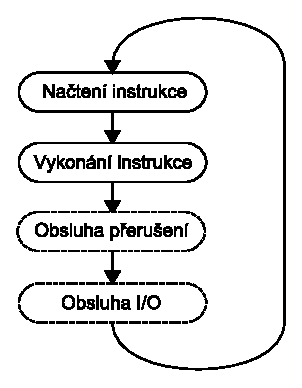
\includegraphics[width=4.5cm,height=6cm]{fig/anal_interpret}
\caption{Interpretační emulace\label{fig:anal_interpreter}}
\end{center}
\end{figure}

% Pamet

\subsection{Paměť}

Instrukce zpracovávané hlavním procesorem obvykle pracují s daty uloženými v
paměti, která je dalším významnou součástí emulovaného systému NEC PCEngine,
stejně jako mapovač, který procesoru umožňuje přistupovat k paměti v celém
rozsahu.

Emulovaná pamět je většinou realizována jako pre-alokované bloky paměti v rámci
platformy, na které emulátor běží. Tyto bloky jsou využívany v situaci, kdy
emulátor v emulovaném programu odchytí pokus o přístup do některého z regionů
paměti jako je RAM, ROM nebo vstupně-výstupní pamět namapovaná zařízeními.
Jednotlivé regiony paměti pak mají nastarost funkce emulující mapovač, které
zajišťují přepočet adresy a aplikaci případných restrikcí přístupu do paměti.

%TODO ukazka kodu?%

% Periferni zarizeni

\subsection{Periferní zařízení}

Systém NEC PCEngine je kromě samotného CPU HuC6280 vybaven řadou periferních
zařízení. Způsob emulace těchto zařízení je závislý na jejich účelu a druhu
činnosti.

Periferní zařízení jsou obvykle představována svým vnitřním stavem (obsah
interní paměti, registrů apod.) a případně uživatelským rozhraním. Často jsou
stejně jako procesor reprezentována datovou strukturou obsahující informace o
vnitřním stavu zařízení, nad kterou operují funkce volané emulačním kódem
procesoru. U zařízení, která disponují zmiňovaným uživatelským rozhraním, je
třeba funkčně zajistit propojení s uživatelským rozhraním emulátoru a patřičnou
konverzi vstupu/výstupu.

V případě systému NEC PCEngine je nutno brát v potaz zejména uživatelské
rozhraní následujících periferních zařízení:

\begin{itemize}
\item port herního ovladače
\item PSG
\item VDC HuC6270, VCE HuC6260
\end{itemize}

U řady zařízení je nutné si uvědomit, že prostředky použité k jejich emulaci
fungují diametrálně odlišně a proto nemusí být vždy nutné emulovat zařízení
zcela přesně. Např. systém vykreslování obrazu pomocí VDC HuC6270 a VCE HuC6260
na obrazovku je v případě emulátoru zcela odlišný (do bitové mapy) než u
původního hardware (na televizní obrazovku) a emulování videovýstupu až po
modulaci analogového signálu vhodného pro RF vstup televizního setu by bylo
zbytečné.

%TODO ukazka kodu?%

% Casovani

\subsection{Časování}

Ve skutečném hardware je časování a synchronizace jednotlivých komponent
zajišťena generátorem hodinových pulzů, který generuje pulzy o konstantní
frekvenci. Hodinový signál je pak vhodně předdělen a dodán jednotlivým
zařízením v systému. Z hlediska emulace existují dva základní přístupy k
časování s ohledem na:

\begin{description}
\item[přesnost] - kód emulátoru zpravidla odpočítává cykly procesoru během
	provádění emulovaného programu a jednotlivé zdroje časových pulzů jsou
	přímo emulovány pomocí služeb platformy, na které emulátor běží. To
	zaručuje dosažení věrohodné rychlosti emulace, pokud to dovolují prostředky
	této platformy. Tento přístup je vhodný spíše tam, kde je kladen důraz na
	průběh emulovaného programu a čas získání výsledku není kritický.

\item[rychlost] - původní zdroje hodinového signálu jsou zcela ignorovány a
	veškerá emulace probíhá maximální možnou rychlostí, kterou udává platforma,
	na které emulátor běží. Tento přístup se často používá při emulaci, kde je
	kladen důraz spíše na výsledek než průběh emulovaného programu.
\end{description}

V případě videoherních konzolí je rychlost provádění programu důležitým
faktorem. Většina herních programů je závislá na postřehu a zručnosti hráče a
rychlost provádění programu je častokrát přímo závislá na taktu procesoru,
protože narozdíl od různorodých konfigurací osobních počítačů je u videoherní
konzole tento parametr pro vývojáře konstantní. Provádění programu určeného pro
procesor s taktovací frekvencí 7.16MHz plnou rychlostí na procesoru s taktovací
frekvencí 2.0GHz bude, i přes výkonostní srážku způsobenou režií emulace, tak
rychlé, že bude program nepoužitelný.

Také je nutné vzít v úvahu fakt, že pro synchronizaci kódu a dění na obrazovce
se u videoherních systémů ve většině případů používá \uv{vertikální
synchronizace}. Do výpočtu časování tedy vstupuje další element - televizní
standard (NTSC nebo PAL), který přesně určuje počet řádků tvořících jeden
snímek, a kolikrát za vteřinu dojde k překreslení celého snímku.

% -----------------------------------------------------------------------------
% Pozadavky na program
% -----------------------------------------------------------------------------

\section{Požadavky na program}\label{chap:anal_requirements}

Úkolem výsledného programu je emulace videoherního systému NEC PCEngine v
rozsahu jeho základní verze, popsané specifikací uvedenou v
kapitole~\ref{chap:spec}, za použití výše popsaných technik a závěrů plynoucích
z rešerše existujících implementací v kapitole~\ref{chap:exist}.

%
% Funkcni pozadavky
%

\subsection{Funkční požadavky}

Výsledný program bude provádět následující činnosti:
\begin{itemize}
	\item načtení obrazu ROM pro NEC PCEngine \\
		\--- načte obraz ROM s programem ze souboru \\
		\--- provede potřebné úpravy obrazu ROM (rozdělení, ořez hlavičky)

	\item emulace zpracování programu \\
		\--- zpracuje interpretačním způsobem program v načteném obrazu ROM

	\item podpora emulace jednotlivých součástí NEC PCEngine \\
		\--- bude emulovat CPU HuC6280 a jeho interní periferní zařízení \\
		\--- bude emulovat základní funkce VDC HuC6270 a VCE HuC6260 \\
		\--- bude emulovat základní funkce PSG\footnote{PSG je fakticky
		součástí CPU HuC6280, ale jedná se o tak rozsáhlou a specifickou
		součást, že ji narozdíl od časovače nebo vstupně-výstupního paralelního
		portu uvádíme separátně.}

	\item interakce s uživatelem \\
		\--- vykreslí aktuální snímek generovaný VDC a VCE \\
		\--- přehraje zvuk generovaný PSG \\
		\--- zpracuje vstup z klávesnice jako vstup z herního ovladače
\end{itemize}

%
% Nefunkcni pozadavky
%

\subsection{Nefunkční požadavky}

Výsledný program bude mít následující vlastnosti:
\begin{itemize}
	\item přenositelnost kódu \\
		\--- bude možné ho sestavit a použít na platformách GNU/Linux a
			Microsoft Windows \\
		\--- bude možné ho jednoduše přenést na další platformy

	\item modularita \\
		\--- bude možné ho jednoduše rozšířit o další emulátory videoherních
			systémů \\
		\--- bude možné ho jednoduše rozšířit o další uživatelská
			rozhraní\footnote{Uživatelským rozhraním je zde myšlena vrstva
			využívající služeb platformy a zprostředkovávající vstup a výstup
			emulátoru uživateli.}

	\item implementační prostředí \\
		\--- bude napsán v jazyce C nebo C++
\end{itemize}

% -----------------------------------------------------------------------------
% Architektura programu
% -----------------------------------------------------------------------------

\section{Architektura programu}\label{chap:anal_architecture}

Architektura programu vychází z principů návrhu otevřeného software pro
operační systém UNIX popsaných v~\cite{Raymond04}. Její základní myšlenkou je
jednoduchost, rozšiřitelnost a oddělení jednotlivých logických částí programu.

Stěžejními prvky architektury programu jsou, přímo na základě nefunkčního
požadavku {\em modularity}, dva typy modulů:

\begin{itemize}
\item moduly emulátorů \\
	\--- zajišťují emulaci videoherních systémů
\item moduly uživatelských rozhraní \\
	\--- zajišťují rozhraní mezi emulátorem a uživatelem (obraz, zvuk, vstup)
\end{itemize}

Tyto moduly mají přesně specifikované rozhraní jak pro komunikaci mezi sebou,
tak pro komunikaci s jádrem programu, které zajišťuje inicializaci správné
dvojice modulů (vždy právě jednoho emulátoru a právě jednoho uživatelského
rozhraní) při spuštění a dále koordinuje jejich práci z hlavní programové
smyčky. Celkový pohled na architekturu programu je naznačen pomocí diagramu
analytického modelu tříd na obr.~\ref{fig:anal_arch}.

%TODO analyticky model
\begin{figure}[ht]
\begin{center}
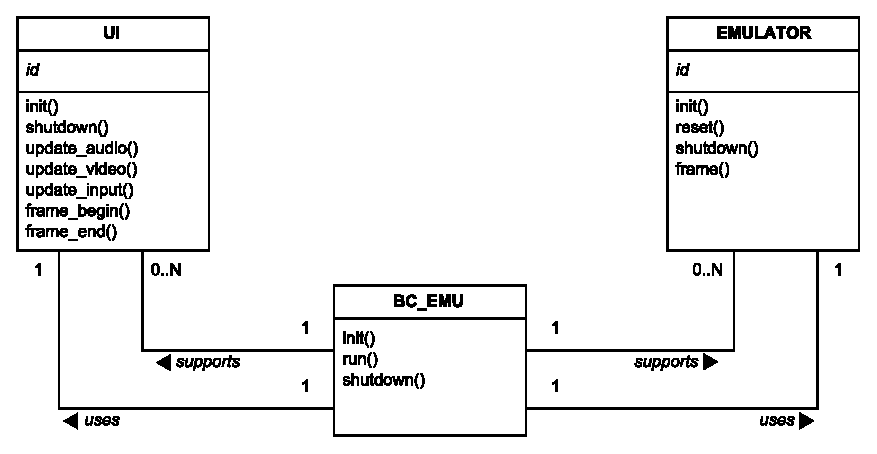
\includegraphics[width=14.2cm,height=7.1cm]{fig/anal_model}
\caption{Architektura programu\label{fig:anal_arch}}
\end{center}
\end{figure}

Kromě možnosti volby z více druhů emulátorů či uživatelských rozhraní, přinese
takto navržená architektura, podpořená možnostmi sestavovacího systému, také
možnost vytvořit personalizovaná sestavení obsahující jen moduly zvolené na
základě potřeb uživatele, nebo restrikcí plynoucích z možností platformy, pro
kterou bude výsledné sestavení programu určeno.

Modularita programu je tak navíc efektivním řešením nefunkčního požadavku na
{\em přenositelnost kódu}. Na platformách, kde nebude možné program sestavit z
důvodu např. závislosti na nedostupné knihovně uživatelského rozhraní, stačí
doimplementovat specifický modul založený na jiné, dostupné knihovně, který
bude \uv{suplovat} přenositelný kód. Poté stačí zavést příslušná omezení
sestavovacího systému pro nucený výběr takového modulu při sestavení pro tuto
platformu.

%
% Modul emulatoru
%

\subsection{Moduly emulátorů}

Emulátory jednotlivých videoherních systémů (v tomto případě NEC PCEngine)
jsou oddělenými moduly, komunikující s ostatními částmi programu pomocí
pevně specifikovaného rozhraní tvořeného několika funkcemi a datovými
strukturami pro výměnu dat. Analytická třída modulu emulátoru je naznačena
pomocí diagramu na obr.~\ref{fig:anal_emu}.

%TODO analyticky model s <<use>> na ty tri rozhrani
\begin{figure}[ht]
\begin{center}
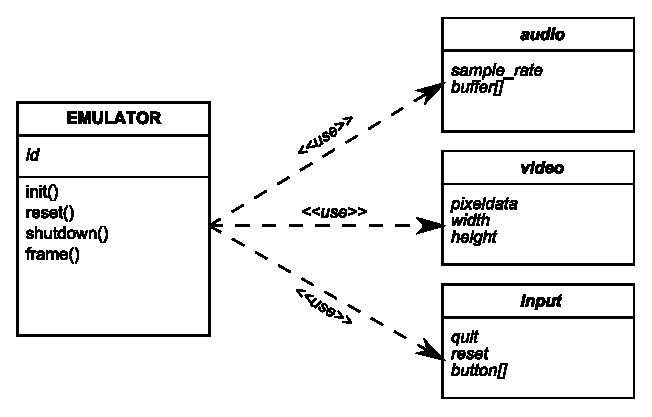
\includegraphics[width=10.5cm,height=6.4cm]{fig/anal_emu}
\caption{Analytická třída modulu emulátoru\label{fig:anal_emu}}
\end{center}
\end{figure}

Veřejné rozhraní modulu emulátoru tvoří, kromě struktur pro výměnu dat s
modulem uživatelského rozhraní (viz.
podsekce~\ref{chap:anal_architecture_struct}), následující funkce:
\begin{itemize}
\item {\it init()} - inicializace emulátoru (konstruktor)
\item {\it reset()} - re-inicializace emulátoru
\item {\it shutdown()} - ukončení činnosti emulátoru (destruktor)
\item {\it frame()} - posun v emulaci o jeden vykreslený snímek
\end{itemize}

Hlavní třídu modulu emulátoru je nutné chápat pouze jako zapouzdření funkčnosti
emulátoru. Je pochopitelné, že kód bude rozsáhlý a složitý a bude reflektovat
řadu specifik architektury konkrétního systému. Proto je architektura za
hranicí tohoto rozhraní zcela ponechána na autorovi konkrétního modulu.

Pro modul emulátoru systému NEC PCEngine je zvolena architektura tvořená čtyřmi
třídami, z nichž každá představuje jeden z funkčních bloků systému (CPU, VDC,
VCE a PSG), jehož vnitřní stav (registry, namapovaná paměť atd.) reprezentuje a
jehož chování emuluje pomocí svých metod.

%
% Moduly uzivatelskych rozhrani
%

\subsection{Moduly uživatelských rozhraní}

Úkolem modulu uživatelského rozhraní je zajistit interakci mezi uživatelem a
modulem emulátoru, resp. v něm běžícího programu. Zpravidla provádí následující
tři činnosti:

\begin{itemize}
\item zobrazit obrazová data získaná od modulu emulátoru
\item přehrát zvuková data získaná od modulu emulátoru
\item zpracovat uživatelský vstup a předat jej modulu emulátoru
\end{itemize}

Požadavek na {\em přenositelnost kódu} komplikuje potřeba programu používat
služby specifické pro určité platformy. Nepochybně největší částí programu
závislou na službách platformy je uživatelské rozhraní. I přes to, že existuje
řada knihoven a rámců zastřešujících práci s uživatelským rozhraním napříč více
platformami, nikdy se nepodaří jednou knihovnou či rámcem pokrýt všechny
možnosti. Oddělení kódu uživatelského rozhraní do modulu, jehož analytická
třída je naznačena pomocí diagramu na obr.~\ref{fig:anal_ui}, je tak logickým
krokem, který je v souladu i s použitím zmíněných knihoven a rámců\footnote{To
je ostatně i případ použité knihovny libSDL (viz. kapitola~\ref{chap:impl}),
díky které bude pro obě platformy dané požadavky, tedy GNU/Linux a Microsoft
Windows, zapotřebí pouze jeden modul uživatelského rozhraní.}.

\begin{figure}[ht]
\begin{center}
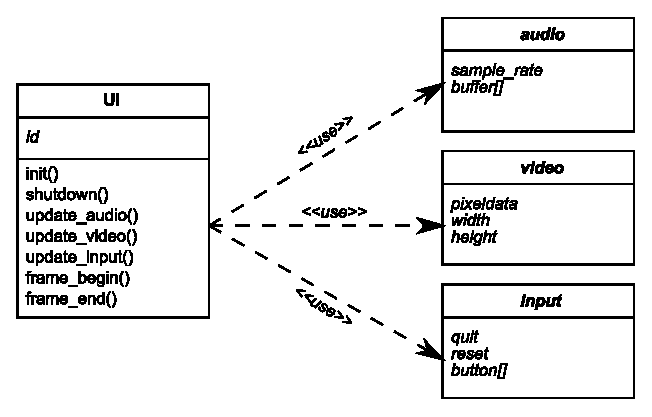
\includegraphics[width=10.5cm,height=6.4cm]{fig/anal_ui}
\caption{Analytická třída modulu uživatelského rozhraní\label{fig:anal_ui}}
\end{center}
\end{figure}

Tímto přístupem navíc docílíme možnosti snadné integrace s různými prostředími.
Modul uživatelského rozhraní nemusí být nutně interaktivní, jednou z mnoha
možností je např. síťová vrstva, která předává a přijímá informace od
vzdáleného klientu. Bez výraznějších úprav tak může výsledný program s tímto
modulem operovat v režimu klient/server po síti.

Moduly uživatelského rozhraní budou se zbytkem programu, podobně jako moduly
emulátorů, komunikovat pomocí pevně specifikovaného rozhraní, které bude
tvořeno, kromě struktur pro výměnu dat s modulem emulátoru (viz.
podsekce~\ref{chap:anal_architecture_struct}), následujícími funkcemi:

\begin{itemize}
\item {\it init()} - inicializace uživatelského rozhraní (konstruktor)
\item {\it shutdown()} - ukončení činnosti uživatelského rozhraní (destruktor)
\item {\it update\_audio()} - aktualizace zvukového výstupu
\item {\it update\_video()} - aktualizace obrazového výstupu
\item {\it update\_input()} - aktualizace vstupu
\item {\it frame\_begin()} - činnost před vykreslením snímku
\item {\it frame\_end()} - činnost po vykreslení snímku
\end{itemize}

Modul uživatelskéh rozhraní obsahuje synchronizační mechanismus tvořený dvojicí
funkcí {\it frame\_begin()} a {\it frame\_end()}. Ten umožňuje provádět kód
před zahájením vykreslení snímku a po jeho ukončení.

Protože mají knihovny a rámce použité pro práci s uživatelským rozhraním
většinou přímý přístup k platformně závislým službám, jako je např. správa
časovačů, je logické umístit mechanismus pro časovou synchronizaci pomocí
těchto služeb právě do modulu uživatelského rozhraní. Kód vykonávaný touto
dvojicí funkcí může např. měřit délku snímku a kompenzovat počet snímků za
sekundu.

%
% Spolecne struktury pro vymenu dat
%

\subsection{Společné struktury pro výměnu
dat}\label{chap:anal_architecture_struct}

Rozhraní obou typů modulů dotváří trojice pomocných struktur určených k výměně
dat v pevně daném formátu. To zajišťuje, že si libovolná, správně provedená
implementace modulu emulátoru \uv{bude rozumět} s libovolnou, správně
provedenou implementací modulu uživatelského rozhraní a naopak. Jedná se o
následující struktury:

\begin{itemize}
\item {\it audio} - pro výměnu informací o zvukovém výstupu (emulátor
	$\rightarrow$ uživatelské rozhraní)
\item {\it video} - pro výměnu informací o obrazovém výstupu (emulátor
	$\rightarrow$ uživatelské rozhraní)
\item {\it input} - pro výměnu informací o stavu vstupu (uživatelské rozhraní
	$\rightarrow$ emulátor)
\end{itemize}
